\documentclass[../../main]{subfiles}

\renewcommand\thesection{\arabic{section}}


\begin{document}

\section{Shift Register System} \label{sec:}

Now let's move on to the controlling of \emph{actuators}. We can simply facilitate
this by using a handful of \emph{shift registers} as we did with multiplexer addressing
circuit. Right now we want to control atmost $16$ different things. So we need a $16$
bit shift register. But $16$ bit shift registers are not readily available in the market.
So we need to cascade available shift registers to build a $16$ bit one.

\subsection{Choosing the Base Shift Register}

We can pick \emph{74LS95} as our base shift register and build from it. It is
a $4$ bit shift register that can be directly driven by \esp as it is a \emph{74LS}
series chip. Refer figures \ref{fig:74ls95Dip} and \ref{fig:74ls95PinDiagram} for
more info about the IC. And table \ref{tbl:74ls95RelventPins} goes through the pins
of \emph{74LS95}.

\alertTip{
    There is no special reason to pick \emph{74LS95} over \emph{74LS96}, as we are using them
    only in their serial mode. Another thing to note is that if you want to control lights
    or actuators other than \emph{fans} or \emph{relays}\footnote{as we are using these
    for.}, you may need to consider shift registers with a secondary set of \emph{storage latches},
    as the \emph{shifting effect}\footnote{if you connect LEDs to these, you can see some of the
    LEDs turning on for a small amount of time as we \emph{shift} the data in.} completely.
}

\begin{center}
    {\begin{minipage}[c] {0.35\textwidth}
        \centering

        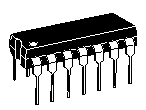
\includegraphics [
        ] {pics/74ls95_dip.pdf}
        \captionof{figure} {
            Dip package of \emph{74LS95}.
            \label{fig:74ls95Dip}
        }

        \includegraphics [
            max width = \IGXMaxWidth,
            max height = \IGXMaxHeight,
            \IGXDefaultOptionalArgs,
        ] {tikzpics/endAbsFourBitShiftRegisterPinout.pdf}
        \captionof{figure} {
            Pin diagram of \emph{74LS95}.
            \label{fig:74ls95PinDiagram}
        }

    \end{minipage}
    \hfill
    \begin{minipage}[c] {0.52\textwidth}

        \centering

        \begin{tabularx} {\linewidth} {
                *{1}{>{\centering\arraybackslash}m{0.3\linewidth}}
                *{1}{>{\centering\arraybackslash}m{0.7\linewidth}}
            }
            \toprule
            Pins & Remarks \\
            \midrule
            \texttt{DS} & Serial in. \\
            \texttt{Q0 - Q3} & Parallel output lines. \\
            \texttt{P0 - P3} & Parallel input lines. \\
            \texttt{S} & Mode select pin. \\
            $\overline{\mbox{\texttt{CP1}}}$ & Clock pin for serial mode. \\
            $\overline{\mbox{\texttt{CP2}}}$ & Clock pin for parallel mode. \\
            \bottomrule
        \end{tabularx}
        \captionof{table} {
            Relevant pins of \emph{74LS95}.
            \label{tbl:74ls95RelventPins}
        }

    \end{minipage}}

\end{center}

\alertNote{
    \emph{74LS95} can be configured in $2$ different modes, \emph{parallel} mode an \emph{serial} mode.
    The mode select pin \texttt{S} determines that mode, if it is low, the chip will be in \emph{serial} mode.
    Otherwise it will be in \emph{parallel} mode. We are simple using the IC in \emph{serial} mode.
}

\subsection{Building a 16 Bit Shift Register}

Now we need $4$ of \emph{74LS95} ICs to accomplish our task. The circuit is really simple, we just
need to cascade these four as in the figure \ref{fig:absSixteenBitShiftRegister}.

\begin{figure}
    \centering
    \includegraphics [
        max width = \IGXMaxWidth,
        max height = \IGXMaxHeight,
        \IGXDefaultOptionalArgs,
    ] {tikzpics/endAbsSixteenBitShiftRegister.pdf}
    \captionof{figure} {$4$ \emph{74LS95} ICs are cascaded to form a $16$ bit shift register.}
    \label{fig:absSixteenBitShiftRegister}
\end{figure}

\alertImportant{
    It is recommended to add a \emph{decoupling capacitor} with a value in between $1 \si{\mu F}$
    to $0.1 \si{\mu F}$ across the Vcc and ground pins. It is not show in figure \ref{fig:absSixteenBitShiftRegister}
    though.
}

\end{document}
